\documentclass{article}      % Specifies the document class

%%%%%%%%%%%%%%%%% CJK 中文版面控制  %%%%%%%%%%%%%%%%%%%%%%%%%%%%%%
%\usepackage{CJK} % CTEX-CJK 中文支持                            %
\usepackage{xeCJK} % seperate the english and chinese		 %
\setCJKmainfont[BoldFont=黑体, ItalicFont=楷体, BoldItalicFont=仿宋]{宋体}
%\usepackage{CJKutf8} % Texlive 中文支持                         %
\usepackage{CJKnumb} %中文序号                                   %
\usepackage{indentfirst} % 中文段落首行缩进                      %
%\setlength\parindent{22pt}       % 段落起始缩进量               %
\renewcommand{\baselinestretch}{1.2} % 中文行间距调整            %
\setlength{\textwidth}{16cm}                                     %
\setlength{\textheight}{24cm}                                    %
\setlength{\topmargin}{-1cm}                                     %
\setlength{\oddsidemargin}{0.1cm}                                %
\setlength{\evensidemargin}{\oddsidemargin}                      %
%%%%%%%%%%%%%%%%%%%%%%%%%%%%%%%%%%%%%%%%%%%%%%%%%%%%%%%%%%%%%%%%%%

\usepackage{amsmath,amsthm,amsfonts,amssymb,bm}          %数学公式
\usepackage{mathrsfs}                                    %英文花体

\usepackage{fontspec} % use to set font
\setCJKmainfont{SimSun}
\XeTeXlinebreaklocale "zh"  % Auto linebreak for chinese
\XeTeXlinebreakskip = 0pt plus 1pt % Auto linebreak for chinese

\usepackage{longtable}                                   %使用长表格

%%%%%%%%%%%%%%%%%%%%%%%%%  参考文献引用 %%%%%%%%%%%%%%%%%%%%%%%%%%%
%%尽量使用 BibTeX(含有超链接,数据库的条目URL即可)                %
%%%%%%%%%%%%%%%%%%%%%%%%%%%%%%%%%%%%%%%%%%%%%%%%%%%%%%%%%%%%%%%%%%%

\usepackage[numbers,sort&compress]{natbib} %紧密排列             %
\usepackage[sectionbib]{chapterbib}        %每章节单独参考文献   %
\usepackage{xcolor}                                        %使用默认允许使用颜色
\usepackage{hypernat}                                                                         %
\usepackage[bookmarksopen=true,pdfstartview=FitH,CJKbookmarks]{hyperref}              %
\hypersetup{bookmarksnumbered,colorlinks,linkcolor=green,citecolor=blue,urlcolor=red}         %
%参考文献含有超链接引用时需要下列宏包,注意与natbib有冲突        %
%\usepackage[dvipdfm]{hyperref}                                  %
%\usepackage{hypernat}                                           %
\newcommand{\upcite}[1]{\hspace{0ex}\textsuperscript{\cite{#1}}} %

%%%%%%%%%%%%%%%%%%%%%%%%%%%%%%%%%%%%%%%%%%%%%%%%%%%%%%%%%%%%%%%%%%%%%%%%%%%%%%%%%%%%%%%%%%%%%%%
%\AtBeginDvi{\special{pdf:tounicode GBK-EUC-UCS2}} %CTEX用dvipdfmx的话,用该命令可以解决      %
%						   %pdf书签的中文乱码问题		      %
%%%%%%%%%%%%%%%%%%%%%%%%%%%%%%%%%%%%%%%%%%%%%%%%%%%%%%%%%%%%%%%%%%%%%%%%%%%%%%%%%%%%%%%%%%%%%%%

%%%%%%%%%%%%%%%%%%%%%  % EPS 图片支持  %%%%%%%%%%%%%%%%%%%%%%%%%%%
\usepackage{graphicx}                                            %
%%%%%%%%%%%%%%%%%%%%%%%%%%%%%%%%%%%%%%%%%%%%%%%%%%%%%%%%%%%%%%%%%%


\begin{document}
%\CJKindent     %在CJK环境中,中文段落起始缩进2个中文字符
\graphicspath{{Figures/}}
%
\renewcommand{\abstractname}{\small{\CJKfamily{hei} 摘\quad 要}} %\CJKfamily{hei} 设置中文字体,字号用\big \small来设
\renewcommand{\refname}{\centering\CJKfamily{hei} 参考文献}
%\renewcommand{\figurename}{\CJKfamily{hei} 图.}
\renewcommand{\figurename}{{\bf Fig}.}
%\renewcommand{\tablename}{\CJKfamily{hei} 表.}
\renewcommand{\tablename}{{\bf Tab}.}

%将图表的Caption写成 图(表) Num. 格式
\makeatletter
\long\def\@makecaption#1#2{%
  \vskip\abovecaptionskip
  \sbox\@tempboxa{#1. #2}%
  \ifdim \wd\@tempboxa >\hsize
    #1. #2\par
  \else
    \global \@minipagefalse
    \hb@xt@\hsize{\hfil\box\@tempboxa\hfil}%
  \fi
  \vskip\belowcaptionskip}
\makeatother

\newcommand{\keywords}[1]{{\hspace{0\ccwd}\small{\CJKfamily{hei} 关键词:}{\hspace{2ex}{#1}}\bigskip}}

%%%%%%%%%%%%%%%%%%中文字体设置%%%%%%%%%%%%%%%%%%%%%%%%%%%
%默认字体 defalut fonts \TeX 是一种排版工具 \\		%
%{\bfseries 粗体 bold \TeX 是一种排版工具} \\		%
%{\CJKfamily{song}宋体 songti \TeX 是一种排版工具} \\	%
%{\CJKfamily{hei} 黑体 heiti \TeX 是一种排版工具} \\	%
%{\CJKfamily{kai} 楷书 kaishu \TeX 是一种排版工具} \\	%
%{\CJKfamily{fs} 仿宋 fangsong \TeX 是一种排版工具} \\	%
%%%%%%%%%%%%%%%%%%%%%%%%%%%%%%%%%%%%%%%%%%%%%%%%%%%%%%%%%

%\addcontentsline{toc}{section}{Bibliography}

%-------------------------------The Title of The Paper-----------------------------------------%
\title{《高性能计算环境下的软件安装》提纲}
%----------------------------------------------------------------------------------------------%

%----------------------The Authors and the address of The Paper--------------------------------%
\author{
\small
%Author1, Author2, Author3\footnote{Communication author's E-mail} \\    %Authors' Names	       %
\small
%(The Address,City Post code)						%Address	       %
}
\date{}					%if necessary					       %
%----------------------------------------------------------------------------------------------%
\maketitle

%-------------------------------------------------------------------------------The Abstract and the keywords of The Paper----------------------------------------------------------------------------%
%\begin{abstract}
%The content of the abstract
%\end{abstract}

%\keywords {Keyword1; Keyword2; Keyword3}
%-----------------------------------------------------------------------------------------------------------------------------------------------------------------------------------------------------%

%----------------------------------------------------------------------------------------The Body Of The Paper----------------------------------------------------------------------------------------%
%Introduction
本书的编撰,侧重于阐述高性能计算机上科学计算软件编译与安装的基本原理、方法和具体应用。当前随着各类计算中心(从大型的国家级超算中心到各科研院所自行搭建的计算服务器)的建设和高性能计算的日益普遍,如何快速有效地在服务器上部署计算软件成为各类计算服务部门的重要任务之一。

各类科学计算软件由于其专业性较高,往往并非一般计算机专业的工程技术人员所熟悉,所以其安装往往由本专业人士完成,然而这些“业内专家”对计算机配置的熟悉程度差别较大,虽然各计算中心一般都配备有简要的技术说明文档(手册),但是对于很多专门的科学计算软件的安装,即使是专业技术人员也视为畏途。

\textcolor{violet}{本书试图打破这一技术壁垒,从实用的角度较为全面地介绍目前高性能计算机上科学计算软件的编译安装的基本过程。全书主要分三部分,紧密围绕高性能计算环境下的科学计算软件的维护与运行}
\section{高性能超级计算平台概述}
本部分围绕超算中心计算环境(包括基本环境和计算环境)

基本环境
\begin{itemize}
	\item 操作系统 \textrm{Linux~}操作系统简介\\
		主要特征
		\begin{enumerate}
			\item \textrm{Linux~}基本思想(1.~一切都是文件;~2.~软件有确定的用途)
			\item 多用户多任务
			\item 支持多种平台
		\end{enumerate}
		\textrm{Linux~}文件系统,包括\\
		普通文件(1.~文本文件;~2.~可执行二进制文件;~3.~数据格式文件)\\
		目录文件、链接文件、设备文件(块设备/字符设备)等\\
		\textrm{Linux~}文件结构,包括\\
		根目录(\textcolor{blue}{/})、\textrm{bin}目录(\textcolor{blue}{/\textrm{bin}})、设备目录(\textcolor{blue}{/\textrm{dev}})、\textrm{etc}目录(\textcolor{blue}{/\textrm{etc}})、库函数目录(\textcolor{blue}{/\textrm{lib}})、\textrm{home~}目录(\textcolor{blue}{/\textrm{home}})、可选目录(\textcolor{blue}{/\textrm{opt}})、用户目录(\textcolor{blue}{/\textrm{usr}})、(\textcolor{blue}{/\textrm{usr}/\textrm{local}})、变量目录(\textcolor{blue}{/\textrm{var}})、设备目录(\textcolor{blue}{/\textrm{root}})
	\item Linux基本命令\\
		对用户来说,熟练掌握\textrm{Linux~}操作系统最重要的体现就是能灵活使用\textrm{Linux~}基本命令并能组织编写\textrm{shell~}脚本,介绍最常用的\textrm{Linux~}基本命令(含选项):\\
		\begin{enumerate}
			\item 最常用的命令,如\\
				\textcolor{red}{\textrm{ls~}}、\textcolor{red}{\textrm{mkdir~}}、\textcolor{red}{\textrm{cd~}}、\textcolor{red}{\textrm{touch~}}、\textcolor{red}{\textrm{echo~}}、\textcolor{red}{\textrm{cat~}}、\textcolor{red}{\textrm{cp~}}、\textcolor{red}{\textrm{mv~}}、\textcolor{red}{\textrm{rm~}}、\textcolor{red}{\textrm{find~}}、\textcolor{red}{\textrm{wc~}}、\textcolor{red}{\textrm{grep~}}、\textcolor{red}{\textrm{tree~}}、\textcolor{red}{\textrm{pwd~}}、\textcolor{red}{\textrm{ln~}}、\textcolor{red}{\textrm{more}}/\textcolor{red}{\textrm{less~}}、\textcolor{red}{\textrm{head}}/\textcolor{red}{\textrm{tail~}}等
			\item 系统管理命令,如\\
				\textcolor{red}{\textrm{who}}、\textcolor{red}{\textrm{hostname~}}、\textcolor{red}{\textrm{top~}}、\textcolor{red}{\textrm{ps~}}、\textcolor{red}{\textrm{du~}}、\textcolor{red}{\textrm{df~}}、\textcolor{red}{\textrm{ifconfig~}}、\textcolor{red}{\textrm{ping~}}、\textcolor{red}{\textrm{alias~}}、\textcolor{red}{\textrm{kill~}}、\textcolor{red}{\textrm{which~}}、\textcolor{red}{\textrm{date~}}等
			\item 管道和文件编辑命令,如\\
				\textcolor{red}{\textrm{|}}、\textcolor{red}{\textrm{sed}}、\textcolor{red}{\textrm{awk}}等
		\end{enumerate}
	\item 文本编辑器vim/emacs
		\begin{enumerate}
			\item \textrm{vim~}编辑器\\
				三种模式:~命令模式、插入模式和编辑模式(详解图\ref{Fig:Vim_Key})
\begin{figure}[h!]
\centering
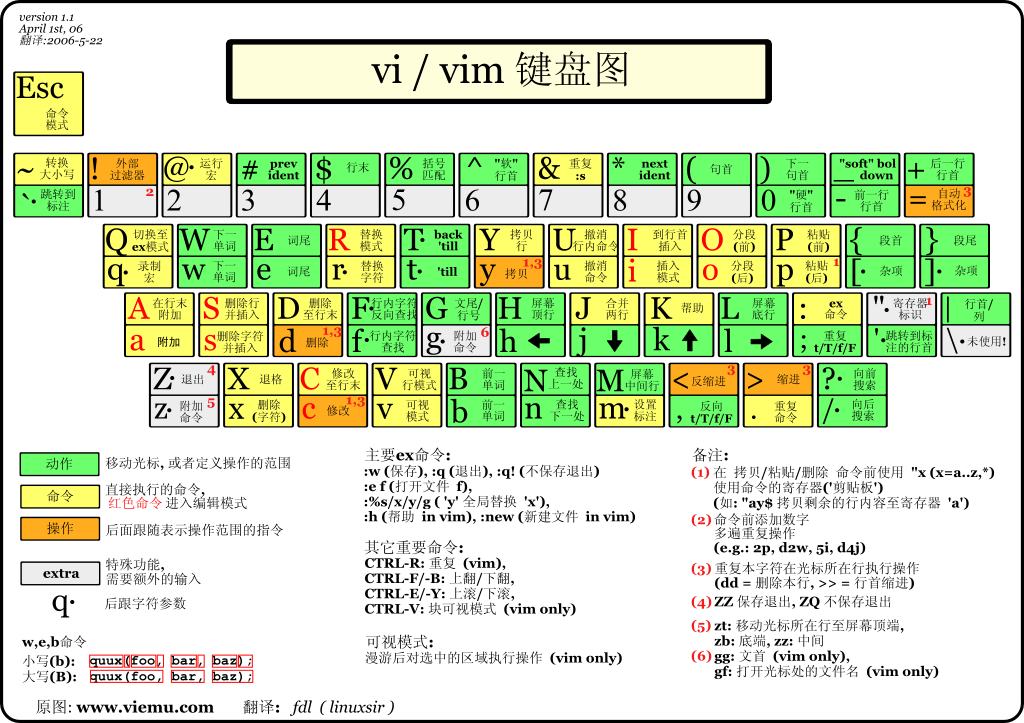
\includegraphics[height=3.25in,width=5.0in,viewport=0 0 1100 750,clip]{Figures/Vim_Key.png}
\caption{\small \textrm{Vim 键盘图}.}%(与文献\cite{EPJB33-47_2003}图1对比)
\label{Fig:Vim_Key}
\end{figure}
			\item \textrm{emacs~}编辑器\\
				\textcolor{magenta}{编辑模式}(主模式和次模式),包括:\\
				文件操作(文件的打开、保存、关闭等)、编辑操作(文件中字符的增删、光标移动、复制、粘贴等)、窗口操作(新开与关闭窗口、垂直或水平关闭窗口等)、目录操作\\
				\textcolor{magenta}{搜索模式},包括:\\
				文件中关键词的快速检索与替换等\\
				\textcolor{magenta}{\textrm{Shell~}执行模式}
				命令操作(执行\textrm{shell}命令)
		\end{enumerate}
\end{itemize}

\section{编译器和库函数}
\textcolor{red}{软件的编译与安装是本书的技术特色。}
\textcolor{blue}{编译的基本过程}:~把用高级程序设计语言书写的源程序,翻译成等价的机器语言格式目标程序。编译过程一般分为四步
\begin{figure}[h!]
\centering
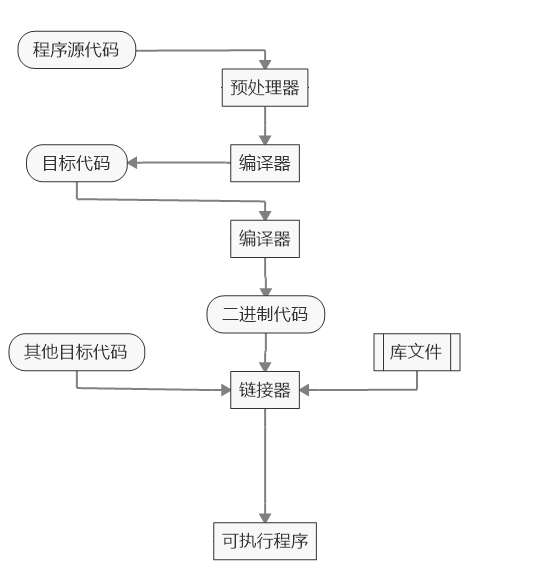
\includegraphics[width=2.0in,height=2.55in,viewport=0 0 490 600,clip]{Figures/compiler_procedure.png}
\caption{\small \textrm{编译过程的四个步骤}.}%(与文献\cite{EPJB33-47_2003}图1对比)
\label{Fig:compiler}
\end{figure}
\begin{itemize}
	\item 预处理,预处理器原本是为协助\textrm{C~}语言工作所设计的,主要完成以下任务:
		\begin{enumerate}
			\item 展开头文件\\
				在写有\textrm{\#~include~ <filename>}或\textrm{\#~include~"filename"}的文件中,将文件\textrm{filename}展开,通俗来说就是将\textrm{fiename}文件中的代码写入到当前文件中;
			\item 宏替换
			\item 去掉注释
			\item 条件编译\\
				即对\textrm{$\#$~ifndef~\#~define~\#~endif}进行判断检查,也正是在这一步,\textrm{\#~ifndef~\#~define~\#~endif}的作用体现出来,即防止头文件被多次重复引用
		\end{enumerate}
	\item 将预处理后的文档转换成汇编语言
		\begin{enumerate}
			\item 编译器在每个文件中保存一个函数地址符表,该表中存储着当前文件内包含的各个函数的地址
			\item 因为这一步要生成汇编代码,即一条一条的指令,而调用函数的代码会被编译成一条\textrm{call}指令,\textrm{call}指令后面跟的是\textrm{jmp}指令的汇编代码地址,而\textrm{jmp}指令后面跟的才是“被调用的函数编译成汇编代码后的第一条指令”的地址,但是给\textrm{call}指令后面补充上地址的工作是在链接的时候做的事情
		\end{enumerate}
	\item 由汇编代码变为目标代码(机器代码)生成\textrm{.o}的二进制文档
	\item 连接目标代码,生成可执行程序\\
		在这个过程中,编译器做的一个重要的事情是将每个文件中\textrm{call}指令后面的地址补充上(方式是从当前文件的函数地址符表中开始找,如果没有,继续向别的文件的函数地址符表中找,找到后填补在\textrm{call}指令后面,如果找不到,则链接失败)

\end{itemize}
科学计算的核心计算软件常用高级语言\textrm{C~}或\textrm{Fortran~}编写(也有用\textrm{Matlab~}编写的,但\textrm{Matlab~}程序自带编译器),本部分分节介绍最常用的编译器和数学库\\
\textcolor{red}{编译器}
\begin{itemize}
	\item \textcolor{blue}{GNU编译器}\\
		\textrm{C/C++~}编译器\textrm{gcc~}:\\
		\textrm{GCC~(GNU Compiler Collection)},是由\textrm{GNU~}开发的编程语言编译器。它是以\textrm{GPL~}许可证所发行的自由软件。\textrm{gcc~}原本作为\textrm{gnu~}操作系统的官方编译器,现已被大多数类\textrm{Unix~}操作系统(如\textrm{Linux}、\textrm{BSD}、\textrm{Mac OS X}等)采纳为标准的编译器\\
		FORTRAN~编译器\textrm{gfortran~}:\\
		\textrm{GFortran~}是\textrm{GNU~}出品的开源编译器,是\textrm{gcc~}的组成部分,也是\textrm{Linux~}平台下最主流的编译器,支持\textrm{F95/2003}部分2008语法。支持\textrm{OpenMP~}并行化计算
	\item \textcolor{blue}{Intel编译器:}\\
		\textrm{C/C++~}编译器\textrm{icc~}/\textrm{FORTRAN~}编译器\textrm{ifort~}:\\
		\textrm{Intel~}编译支持\textrm{IA-32}、\textrm{Intel~64}、\textrm{Itanium~2}、\textrm{Intel~Atom~}处理器和某些非\textrm{Intel~}的兼容处理器(如某些\textrm{AMD~}处理器)。\textrm{Intel~Compiler~}进一步支持\textrm{OpenMP~3.0~}和适用于对称多处理的自动并行化
	\item \textcolor{blue}{PGI编译器}\\
		C/C++~编译器\textrm{pgcc~}/FORTRAN~编译器\textrm{pgf90~}:\\
		\textrm{PGI~Compiler}由\textrm{Portland~}公司开发的编译器,支持\textrm{AMD~Opteron}/\textrm{Althon~}处理器、\textrm{Intel~Xeon~}处理器等,在\textrm{Opteron~}上同时支持\textrm{32-bit~}和\textrm{64-bit~},支持\textrm{Linux~}、\textrm{Windows~},支持\textrm{C/C++}、\textrm{Fortran77}、\textrm{Fortran90/95}、\textrm{HPF~}支持多线程和\textrm{OpenMP~}\\
		\textrm{PGI~Compiler~}需要购买,但可以从网上得到15天试用版本\url{http://www.pgroup.com}
\end{itemize}

\textcolor{red}{\textrm{OPENMP~}与\textrm{MPI~}}
\begin{itemize}
	\item \textrm{OpenMP(Open Multiprocessing)}是一种应用程序界面(\textrm{API},即\textrm{Application Program Interface}),是一种并行的实现和方法,在节点内(多核\textrm{SMP~})执行的基于共享内存的编程模型型,可用于共享内存并行系统的多线程程序设计的一套指导性注释(\textrm{Compiler Directive}) \textrm{OpenMP~}更适合单台计算机共享内存结构上的并行计算。由于使用线程间共享内存的方式协调并行计算,它在多核/多CPU结构上的效率很高、内存开销小、编程语句简洁直观,因此编程容易、编译器实现也容易(现在的\textrm{C/C++}、\textrm{Fortran~}编译器基本上都内置\textrm{OpenMP}支持)\\
\textrm{OpenMP~}最大的缺点是只能在单台主机上工作,不能用于多台主机间的并行计算\\
	\item \textrm{MPI(Message Passing Interface)},是在分布式内存\textrm{distributed-memory~}之间实现信息通讯的一种规范/标准/协议(\textrm{standard})。它是一个库,不是一门语言。可以被\textrm{fortran~}、\textrm{c/c++~}等调用。\textrm{MPI~}允许静态任务调度,显示并行提供了良好的性能和移植性,用\textrm{MPI~}编写的程序可直接在多核集群上运行。在集群系统中,集群的各节点之间可以采用\textrm{MPI~}编程模型进行程序设计,每个节点都有自己的内存,可以对本地的指令和数据直接进行访问,各节点之间通过互联网络进行消息传递,这样设计具有很好的可移植性,完备的异步通信功能,较强的可扩展性等优点。\\
\textrm{MPI~}模型存在一些不足,包括: 程序的分解、开发和调试相对困难,而且通常要求对代码做大量的改动;通信会造成很大的开销,为了最小化延迟,通常需要大的代码粒度;细粒度的并行会引发大量的通信;动态负载平衡困难;并行化改进需要大量地修改原有的串行代码,调试难度比较大
\end{itemize}

\textcolor{red}{\textrm{MPICH~}与\textrm{OPENMPI~}}\\
\textrm{openMPI(open Message Passing Interface)}和\textrm{MPICH~}都是采用MPI标准,在并行计算中,实现节点间通信的开源软件。各自有各自的函数,指令和库。此外MPI的实现还有\textrm{MPI-1~},\textrm{MPI-2~}等等\\
\textcolor{red}{$\ast$可选章节:~}
\begin{itemize}
	\item Openmpi~编译器的编译选项
	\item MPICH2/3~编译器的编译选项
\end{itemize}
\textcolor{red}{数学库和FFTW库}\\
\begin{itemize}
	\item \textrm{BLAS~}库\\
		\textrm{BLAS},即基础线性代数子程序库,拥有大量已经编写好的关于线性代数运算的程序,是数值计算最重要的数学函数库,包含3个\textrm{Level~}的线性代数运算,都是以\textrm{Fortran~}语言写的高效率程序。\textrm{BLAS Level 1-3} 分别是向量-向量运算,矩阵-向量运算和矩阵-矩阵运算,从计算复杂度\textrm{O(n)~}向\textrm{O(n$^3$)}过渡
	\item \textrm{ATLAS~}库\\
		\textrm{ATLAS~}是\textrm{BLAS~}线性算法库的优化版本
	\item \textrm{LAPACK}库\\
		\textrm{LAPACK~}库,是在\textrm{BLAS~}基础上发展起来的,针对线性代数方程组,线性最小二乘问题和矩阵特征值问题求解的函数库,用\textrm{Fortran~}语言编写,\textrm{LAPACK~}提供了可用于诸如求解多元线性方程组、线性系统方程组的最小平方解、计算特征向量、用于计算矩阵\textrm{QR~}分解的\textrm{Householder~}转换、以及奇异值分解等问题。 在\textrm{NetLib~}提供了\textrm{API~}简化的\textrm{Fortran 95~}版本的\textrm{LAPACK95~}。\textrm{LAPACK~}以\textrm{BSD~}授权的方法发布
	\item \textrm{Intel\_MKL}库\\
		\textrm{Inte\_mkl(Intel Math Kernel Library)}是\textrm{Intel~}的数学核心函数库, 提供经过高度优化和大量线程化处理的数学函数,面向性能要求极高的科学、工程及金融等领域的应用。针对当前多核\textrm{x86~}平台进行了深入而全面的优化,同时将不断针对未来平台进行优化,以确保应用能够从最新架构的进步中最大限度获益。\\
		\textrm{MKL~}提供的线性代数库函数包括:\\
		\begin{enumerate}
			\item \textrm{BLAS~}:~  \textrm{BLAS Level 1, BLAS Level 2, BLAS Level 3, Sparse BLAS}
			\item \textrm{LAPACK~}:~ 与\textrm{Netlib~}的新\textrm{LAPACK~3.1}函数接口兼容
			\item \textrm{ScaLAPACK~}:~与\textrm{Netlib Scalapack~}接口兼容
				\textrm{MKL~}提供的\textrm{wrapper~}函数为C的源代码,这些\textrm{wrapper~}函数将\textrm{FFTW~}的接口转换为\textrm{Intel MKL}的\textrm{DFTI Fourier~}函数调用。 基于\textrm{FFTW~}接口的程序,不再需要修改源代码,就能够使用\textrm{MKL~}的\textrm{DFT~(discrete Fourier transform)}变换函数。由于\textrm{FFTW~}与\textrm{MKL~}的\textrm{DFTI~}的函数功能不完全相同,用户在使用\textrm{MKL~}的\textrm{Wrapper~}函数去替代\textrm{FFTW~}的时候,会有一些具体的限制
		\end{enumerate}
	\item FFTW2/3库
		\textrm{FFTW~}是由\textrm{MIT~}开发的,广泛使用的\textrm{Fourier~}变换函数库,用标准\textrm{C~}语言编写。\textrm{Intel~}的数学库和\textrm{Scilib}(类似于\textrm{Matlab~}的科学计算软件)都使用\textrm{FFTW~}做\textrm{FFT~}计算
\end{itemize}

\textcolor{red}{程序维护工具make}\\
\textrm{make}是一种维护程序文件的工具,它根据程序中模块的修改情况,自动判断对应哪些模块需要重新编译,保证软件由最新的模块组成。\textcolor{green}{\textrm{make}}命令操作由目录中名为\textcolor{blue}{\textrm{Makefile}}或\textcolor{blue}{\textrm{makefile}}决定,文件描述了系统中模块之间的相互依赖关系,以及产生目标文件所需执行的命令
\begin{itemize}
	\item 依赖关系\\
		\textrm{make~}程序自动生成和维护通常可执行模块或应用程序的“目标”,“目标”状态取决于依赖的模块的状态
	\item 相关行\\
		\textcolor{purple}{相关行}描述\textcolor{purple}{目标}、\textcolor{purple}{模块}和\textcolor{purple}{命令}的关系\\
		\textcolor{purple}{\textrm{target}}:$[$\textcolor{purple}{\textrm{dependent}}$]$\\
		\indent\;\;\;\;\;\;\textcolor{purple}{\textrm{command}}\\
		\indent\;\;\;\;\;\;\textcolor{purple}{\textrm{command}}
\end{itemize}
\textcolor{red}{$\ast$可选章节\\CMake}

\section{高性能计算集群作业管理系统}
本部分分节介绍各种集群作业管理系统\\
作业管理系统的功能
\begin{itemize}
	\item \textcolor{brown}{资源管理器}:~管理超算系统的硬件资源及认证信息等
	\item \textcolor{brown}{队列管理器}:~管理当前已经提交但还未完成的作业
	\item \textcolor{brown}{调度器}:~为作业分配资源
\end{itemize}
作业管理的主要作用
\begin{itemize}
	\item 根据用户作业提出的需求分配对应的资源给作业,告诉作业给它分配哪些节点等
	\item 避免作业之间无序干扰,尽量让整个系统的负载一致
	\item 保证用户占用资源的长期内公平
\end{itemize}
\begin{enumerate}
	\item PBS~\\
		\textrm{PBS~}最初由\textrm{NASA~}的\textrm{Ames~}研究中心开发, 为了提供一个能满足异构计算网络需要的软件包,特别是满足高性能计算的需要。它力求提供对批处理的初始化和调度执行的控制,允许作业在不同主机间的路由\\
		\textrm{PBS~}是功能最为齐全,历史最悠久,支持最广泛的本地集群调度器之一。\textrm{PBS~}的目前包括\textrm{openPBS},\textrm{PBS~Pro}和\textrm{Torque~}三个主要分支。其中\textrm{OpenPBS~}是最早的\textrm{PBS~}系统,目前已经没有太多后续开发,\textrm{PBS~pro}是\textrm{PBS~}的商业版本,功能最为丰富。\textrm{Torque~}是\textrm{Clustering~}公司继承\textrm{OpenPBS~},并给与后续支持的一个开源版本
	\item LSF~\\
		\textrm{IBM~}公司的\textrm{Platform LSF~}是强大的工作负载管理平台,可以进行计算资源的调度与管理,可用于要求苛刻的分布式\textrm{HPC~}环境。它提供由策略推动的一组全面的智能调度功能,支持您利用所有计算基础架构资源并确保最优的应用程序性能。\textrm{Platform LSF~}拥有一系列可选附加组件,旨在帮助其实现工作负载管理、进而提升用户生产效率
	\item \textrm{SLURM~(Simple Linux Utility Resource Management)}\\
		\textrm{SLURM~}是一种可用于大型计算节点集群的高度可伸缩和容错的集群管理器和作业调度系统。\textrm{SLURM~}维护着一个待处理工作的队列并管理此工作的整体资源利用。它还以一种排他或非排他的方式管理可用的计算节点(取决于资源的需求)。\textrm{SLURM~}将作业分发给一组已分配的节点来执行工作并监视平行作业至其完成\\
		本质上,\textrm{SLURM~}是一个强健的集群管理器(更关注于对功能丰富性的需求方面),它高度可移植、可伸缩至大型节点集群、容错好,而且更重要的是它是开源的。\textrm{SLURM~}最早是一个开源的资源管理器,由几家公司(包括\textrm{Lawrence Livermore National Laboratory})协作开发。如今,\textrm{SLURM~}已经成为了很多最强大的超级计算机上使用的领先资源管理器
\begin{figure}[h!]
\centering
\includegraphics[height=3.25in,width=5.0in]{Figures/Slurm-1.gif}
\caption{\small \textrm{SLURM~}架构的高级别视图.}%(与文献\cite{EPJB33-47_2003}图1对比)
\label{Fig:Slurm}
\end{figure}
	\item CONTOR~\\
		\textrm{CONTOR~}是由美国威斯康星大学开发的机群作业管理系统,该项目得到美国政府(国防部、能源部、美国国家宇航局、国家科学基金)和众多企业(\textrm{AT\&T, IBM, Intel, Microsoft, UW-Madison})的资助。)\\
		\textrm{CONTOR~}管理一个专用于某类计算的工作站群(机群),它能有效地利用网络中能相互通讯的工作站的计算力,创造一个高吞吐量计算\textrm{HTC~}环境,这些机器可能分布于不同的地域,分别属于不同的用户。\textrm{CONTOR~}是专门用于管理计算密集型(\textrm{compute-intensive})分布式机群作业的批处理系统
\end{enumerate}

关于各类作业管理系统的简介和使用,\textcolor{red}{针对上述各类作业管理系统,请完善:~\\
\begin{itemize}
	\item 作业管理系统的脚本管理(常见变量)
	\item 作业管理系统的命令
\end{itemize}}
%-------------------The Figure Of The Paper------------------
%\begin{figure}[h!]
%\centering
%\includegraphics[height=3.35in,width=2.85in,viewport=0 0 400 475,clip]{PbTe_Band_SO.eps}
%\hspace{0.5in}
%\includegraphics[height=3.35in,width=2.85in,viewport=0 0 400 475,clip]{EuTe_Band_SO.eps}
%\caption{\small Band Structure of PbTe (a) and EuTe (b).}%(与文献\cite{EPJB33-47_2003}图1对比)
%\label{Pb:EuTe-Band_struct}
%\end{figure}

%-------------------The Equation Of The Paper-----------------
%\begin{equation}
%\varepsilon_1(\omega)=1+\frac2{\pi}\mathscr P\int_0^{+\infty}\frac{\omega'\varepsilon_2(\omega')}{\omega'^2-\omega^2}d\omega'
%\label{eq:magno-1}
%\end{equation}

%\begin{equation} 
%\begin{split}
%\varepsilon_2(\omega)&=\frac{e^2}{2\pi m^2\omega^2}\sum_{c,v}\int_{BZ}d{\vec k}\left|\vec e\cdot\vec M_{cv}(\vec k)\right|^2\delta [E_{cv}(\vec k)-\hbar\omega] \\
% &= \frac{e^2}{2\pi m^2\omega^2}\sum_{c,v}\int_{E_{cv}(\vec k=\hbar\omega)}\left|\vec e\cdot\vec M_{cv}(\vec k)\right|^2\dfrac{dS}{\nabla_{\vec k}E_{cv}(\vec k)}
% \end{split}
%\label{eq:magno-2}
%\end{equation}

%-------------------The Table Of The Paper----------------------
%\begin{table}[!h]
%\tabcolsep 0pt \vspace*{-12pt}
%\caption{The representative $\vec k$ points contributing to $\sigma_2^{xy}$ of interband transition in EuTe around 2.5 eV.}
%\label{Table-EuTe_Sigma}
%\begin{minipage}{\textwidth}
%%\begin{center}
%\centering
%\def\temptablewidth{1.01\textwidth}
%\rule{\temptablewidth}{1pt}
%\begin{tabular*} {\temptablewidth}{@{\extracolsep{\fill}}cccccc}

%-------------------------------------------------------------------------------------------------------------------------
%&Peak (eV)  & {$\vec k$}-point            &Band{$_v$} to Band{$_c$}  &Transition Orbital
%Components\footnote{波函数主要成分后的括号中,$5s$、$5p$和$5p$、$4f$、$5d$分别指碲和铕的原子轨道。} &Gap (eV)   \\ \hline
%-------------------------------------------------------------------------------------------------------------------------
%&2.35       &(0,0,0)         &33$\rightarrow$34    &$4f$(31.58)$5p$(38.69)$\rightarrow$$5p$      &2.142   \\% \cline{3-7}
%&       &(0,0,0)         &33$\rightarrow$34    &$4f$(31.58)$5p$(38.69)$\rightarrow$$5p$      &2.142   \\% \cline{3-7}
%-------------------------------------------------------------------------------------------------------------------------

%\end{tabular*}
%\rule{\temptablewidth}{1pt}\\
%%\end{center}
%\end{minipage}
%\end{table}

%-------------------The Long Table Of The Paper--------------------
%\begin{small}
%%\begin{minipage}{\textwidth}
%%\begin{longtable}[l]{|c|c|cc|c|c|} %[c]指定长表格对齐方式
%\begin{longtable}[c]{|c|c|p{1.9cm}p{4.6cm}|c|c|}
%\caption{Assignment for the peaks of EuB$_6$}
%\label{tab:EuB6-1}\\ %\\长表格的caption中换行不可少
%\hline
%%
%--------------------------------------------------------------------------------------------------------------------------------
%\multicolumn{2}{|c|}{\bfseries$\sigma_1(\omega)$谱峰}&\multicolumn{4}{c|}{\bfseries部分重要能带间电子跃迁\footnotemark}\\ \hline
%\endfirsthead
%--------------------------------------------------------------------------------------------------------------------------------
%%
%\multicolumn{6}{r}{\it 续表}\\
%\hline
%--------------------------------------------------------------------------------------------------------------------------------
%标记 &峰位(eV) &\multicolumn{2}{c|}{有关电子跃迁} &gap(eV)  &\multicolumn{1}{c|}{经验指认} \\ \hline
%\endhead
%--------------------------------------------------------------------------------------------------------------------------------
%%
%\multicolumn{6}{r}{\it 续下页}\\
%\endfoot
%\hline
%--------------------------------------------------------------------------------------------------------------------------------
%%
%%\hlinewd{0.5$p$t}
%\endlastfoot
%--------------------------------------------------------------------------------------------------------------------------------
%%
%% Stuff from here to \endlastfoot goes at bottom of last page.
%%
%--------------------------------------------------------------------------------------------------------------------------------
%标记 &峰位(eV)\footnotetext{见正文说明。} &\multicolumn{2}{c|}{有关电子跃迁\footnotemark} &gap(eV) &\multicolumn{1}{c|}{经验指认\upcite{PRB46-12196_1992}}\\ \hline
%--------------------------------------------------------------------------------------------------------------------------------
%
%     &0.07 &\multicolumn{2}{c|}{电子群体激发$\uparrow$} &--- &电子群\\ \cline{2-5}
%\raisebox{2.3ex}[0pt]{$\omega_f$} &0.1 &\multicolumn{2}{c|}{电子群体激发$\downarrow$} &--- &体激发\\ \hline
%--------------------------------------------------------------------------------------------------------------------------------
%
%     &1.50 &\raisebox{-2ex}[0pt][0pt]{20-22(0,1,4)} &2$p$(10.4)4$f$(74.9)$\rightarrow$ &\raisebox{-2ex}[0pt][0pt]{1.47} &\\%\cline{3-5}
%     &1.50$^\ast$ & &2$p$(17.5)5$d_{\mathrm E}$(14.0)$\uparrow$ & &4$f$$\rightarrow$5$d_{\mathrm E}$\\ \cline{3-5}
%     \raisebox{2.3ex}[0pt][0pt]{$a$} &(1.0$^\dagger$) &\raisebox{-2ex}[0pt][0pt]{20-22(1,2,6)} &\raisebox{-2ex}[0pt][0pt]{4$f$(89.9)$\rightarrow$2$p$(18.7)5$d_{\mathrm E}$(13.9)$\uparrow$}\footnotetext{波函数主要成分后的括号中,2$s$、2$p$和5$p$、4$f$、5$d$、6$s$分别指硼和铕的原子轨道;5$d_{\mathrm E}$、5$d_{\mathrm T}$分别指铕的(5$d_{z^2}$,5$d_{x^2-y^2}$和5$d_{xy}$,5$d_{xz}$,5$d_{yz}$)轨道,5$d_{\mathrm{ET}}$(或5$d_{\mathrm{TE}}$)则指5个5$d$轨道成分都有,成分大的用脚标的第一个字母标示;2$ps$(或2$sp$)表示同时含有硼2$s$、2$p$轨道成分,成分大的用第一个字母标示。$\uparrow$和$\downarrow$分别标示$\alpha$和$\beta$自旋电子跃迁。} &\raisebox{-2ex}[0pt][0pt]{1.56} &激子跃迁。 \\%\cline{3-5}
%     &(1.3$^\dagger$) & & & &\\ \hline
%--------------------------------------------------------------------------------------------------------------------------------

%     & &\raisebox{-2ex}[0pt][0pt]{19-22(0,0,1)} &2$p$(37.6)5$d_{\mathrm T}$(4.5)4$f$(6.7)$\rightarrow$ & & \\\nopagebreak %\cline{3-5}
%     & & &2$p$(24.2)5$d_{\mathrm E}$(10.8)4$f$(5.1)$\uparrow$ &\raisebox{2ex}[0pt][0pt]{2.78} &a、b、c峰可能 \\ \cline{3-5}
%     & &\raisebox{-2ex}[0pt][0pt]{20-29(0,1,1)} &2$p$(35.7)5$d_{\mathrm T}$(4.8)4$f$(10.0)$\rightarrow$ & &包含有复杂的\\ \nopagebreak%\cline{3-5}
%     &2.90 & &2$p$(23.2)5$d_{\mathrm E}$(13.2)4$f$(3.8)$\uparrow$ &\raisebox{2ex}[0pt][0pt]{2.92} &强激子峰。$^{\ast\ast}$\\ \cline{3-5}
%$b$  &2.90$^\ast$ &\raisebox{-2ex}[0pt][0pt]{19-22(0,1,1)} &2$p$(33.9)4$f$(15.5)$\rightarrow$ & &B2$s$-2$p$的价带 \\ \nopagebreak%\cline{3-5}
%     &3.0 & &2$p$(23.2)5$d_{\mathrm E}$(13.2)4$f$(4.8)$\uparrow$ &\raisebox{2ex}[0pt][0pt]{2.94} &顶$\rightarrow$B2$s$-2$p$导\\ \cline{3-5}
%     & &12-15(0,1,2) &2$p$(39.3)$\rightarrow$2$p$(25.2)5$d_{\mathrm E}$(8.6)$\downarrow$ &2.83 &带底跃迁。\\ \cline{3-5}
%     & &14-15(1,1,1) &2$p$(42.5)$\rightarrow$2$p$(29.1)5$d_{\mathrm E}$(7.0)$\downarrow$ &2.96 & \\\cline{3-5}
%     & &13-15(0,1,1) &2$p$(40.4)$\rightarrow$2$p$(28.9)5$d_{\mathrm E}$(6.6)$\downarrow$ &2.98 & \\ \hline
%--------------------------------------------------------------------------------------------------------------------------------
%%\hline
%%\hlinewd{0.5$p$t}
%\end{longtable}
%%\end{minipage}{\textwidth}
%%\setlength{\unitlength}{1cm}
%%\begin{picture}(0.5,2.0)
%%  \put(-0.02,1.93){$^{1)}$}
%%  \put(-0.02,1.43){$^{2)}$}
%%\put(0.25,1.0){\parbox[h]{14.2cm}{\small{\\}}
%%\put(-0.25,2.3){\line(1,0){15}}
%%\end{picture}
%\end{small}

%-----------------------------------------------------------------------------------------------------------------------------------------------------------------------------------------------------%


%--------------------------------------------------------------------------The Biblography of The Paper-----------------------------------------------------------------%
%\newpage																				%
%-----------------------------------------------------------------------------------------------------------------------------------------------------------------------%
%\begin{thebibliography}{99}																		%
%%\bibitem{PRL58-65_1987}H.Feil, C. Haas, {\it Phys. Rev. Lett.} {\bf 58}, 65 (1987).											%
%\end{thebibliography}																			%
%-----------------------------------------------------------------------------------------------------------------------------------------------------------------------%
%																					%
\phantomsection\addcontentsline{toc}{section}{Bibliography}	 %直接调用\addcontentsline命令可能导致超链指向不准确,一般需要在之前调用一次\phantomsection命令加以修正	%
\bibliography{ref/Myref}																			%
\bibliographystyle{ref/mybib}																		%
%  \nocite{*}																				%
%-----------------------------------------------------------------------------------------------------------------------------------------------------------------------%

\clearpage     %\end{CJK} 前加上\clearpage是CJK的要求
\end{document}
